\documentclass[11pt]{article}
\linespread{1.25}

\usepackage[top = 2cm, right=2cm, left=2cm]{geometry}
\usepackage{graphicx}

\usepackage[section]{placeins}
\usepackage[hidelinks, urlcolor=blue]{hyperref}
\usepackage{float} % for image position in exatly where you want
\usepackage[perpage, stable]{footmisc}
\usepackage{amsmath}
\usepackage{titling}

\usepackage{xepersian}
\settextfont{B Nazanin}
\setlatinmonofont{CMU Serif}
%\setlatinmonofont{Times New Roman}
\setlatintextfont{Times New Roman}

% Set Latin Modern font for the bullets in itemizea
\newfontfamily\latinbullet{Latin Modern Roman}





% Commands
\newcommand{\column}[1]{\lr{\textit{#1}}}
\renewcommand{\labelitemi}{{\latinbullet\textbullet}} % Use the bullet from Latin Modern font

% Custom title page setup
\makeatletter
\def\maketitle{
	\begin{titlepage}
		\begin{center}
			\vspace*{2cm}
			
			{\Large\bfseries درس داده کاوی\par}
			\vspace{2cm}
			
			{\Huge\bfseries گزارش تکلیف\\
				\lr{Image Compression with K-Means}\par}
			\vspace{3cm}
			
			{\large\bfseries استاد درس:\par}
			{\large دکتر قاضی زاده\par}
			\vspace{1.5cm}
			
			{\large\bfseries نگارش:\par}
			{\large امیرحسین ابوالحسنی\par}
			{\large شماره دانشجویی: 400405003\par}
			\vspace{2cm}
			
			\vfill  % pushes the date to bottom
			
			{\large\bfseries پاییز \lr{1403}}
			
		\end{center}
	\end{titlepage}
	\setcounter{page}{1}
}
\makeatother

\begin{document}
	\maketitle
	\tableofcontents
	\newpage
	\section{مقدمه}
	خوشه بندی یک عمل بدون نظارت
	\footnote{\lr{Unsupervised}}
	می‌باشد.
	یکی از کاربردهای مشهور آن، انجام فشرده سازی تصویر است که اولین با استفاده از الگوریتم 
\lr{K-Means}
صورت گرفت. این الگوریتم یکی از مشهور‌ترین الگوریتم‌های حوزه خوشه بندی می‌باشد که همچنان استفاده بسیار زیادی از آن می شود.\\
در این تکلیف به فشرده سازی تصویر با الگوریتم \lr{K-Means} می‌پردازیم.
\section{کتابخانه‌های مهم}
\begin{itemize}
	\item \lr{Scikit-Learn}: مورد استفاده برای انجام خوشه بندی با الگوریتم
	\lr{K-Means}
	\item \lr{Numpy}: مورد استفاده برای تغییر ابعاد تصویر و کار با ماتریس تصویر
	\item \lr{PIL(Pillow)}: مورد استفاده برای باز کردن و ذخیره کردن تصویر
	\item \lr{Matplotlib}: مورد استفاده برای نشان دادن تصاویر
\end{itemize}
\section{شیوه کلی حل}
هدف، خوشه بندی روی رنگ‌های تصویر است. در ابتدا تصویر را به یک تنسور سه بعدی تبدیل می‌کنیم. سپس این تنسور سه بعدی که دارای ابعاد 
$(width, height, channel)$
می‌باشد را به یک ماتریس به ابعاد
 $(width \times height, channel)$ 
 تبدیل میکنیم، بدین صورت که هر ردیف این ماتریس، نشان دهنده مقادیر $(R,G,B)$ می‌باشد(جدول
\ref{tbl: x format}
).
\begin{table}[H]
	\centering
	\begin{tabular}{|c|c|c|c|}
		\hline
		شماره پیکسل (ایندکس) & \lr{R} & \lr{G} & \lr{B}\\
		\hline
		1 & 23 & 31 &‌186\\
		2 & 47 & 94 &‌216\\
		3 & 23 & 31 &‌186\\
		\vdots & \vdots & \vdots &‌\vdots\\
		\hline
	\end{tabular}
	\caption{ماتریس ورودی الگوریتم خوشه بندی}
	\label{tbl: x format}
\end{table}

سپس خروجی الگوریتم خوشه بندی را به تصویر تبدیل می‌کنیم، این خروجی همان تصویر فشرده شده می‌باشد.
\newpage
\section{نتایچ}
\section{مقایسه تصاویر با مقادیر $k$‌ متفاوت}
تصویر زیر نشان دهنده انجام الگوریتم با مقادیر
$k = 2, 4, 8, 16, 32$
روی تصویر می باشد.(شکل 
\ref{fig: dif k}
)
\begin{figure}[H]
	\centering
	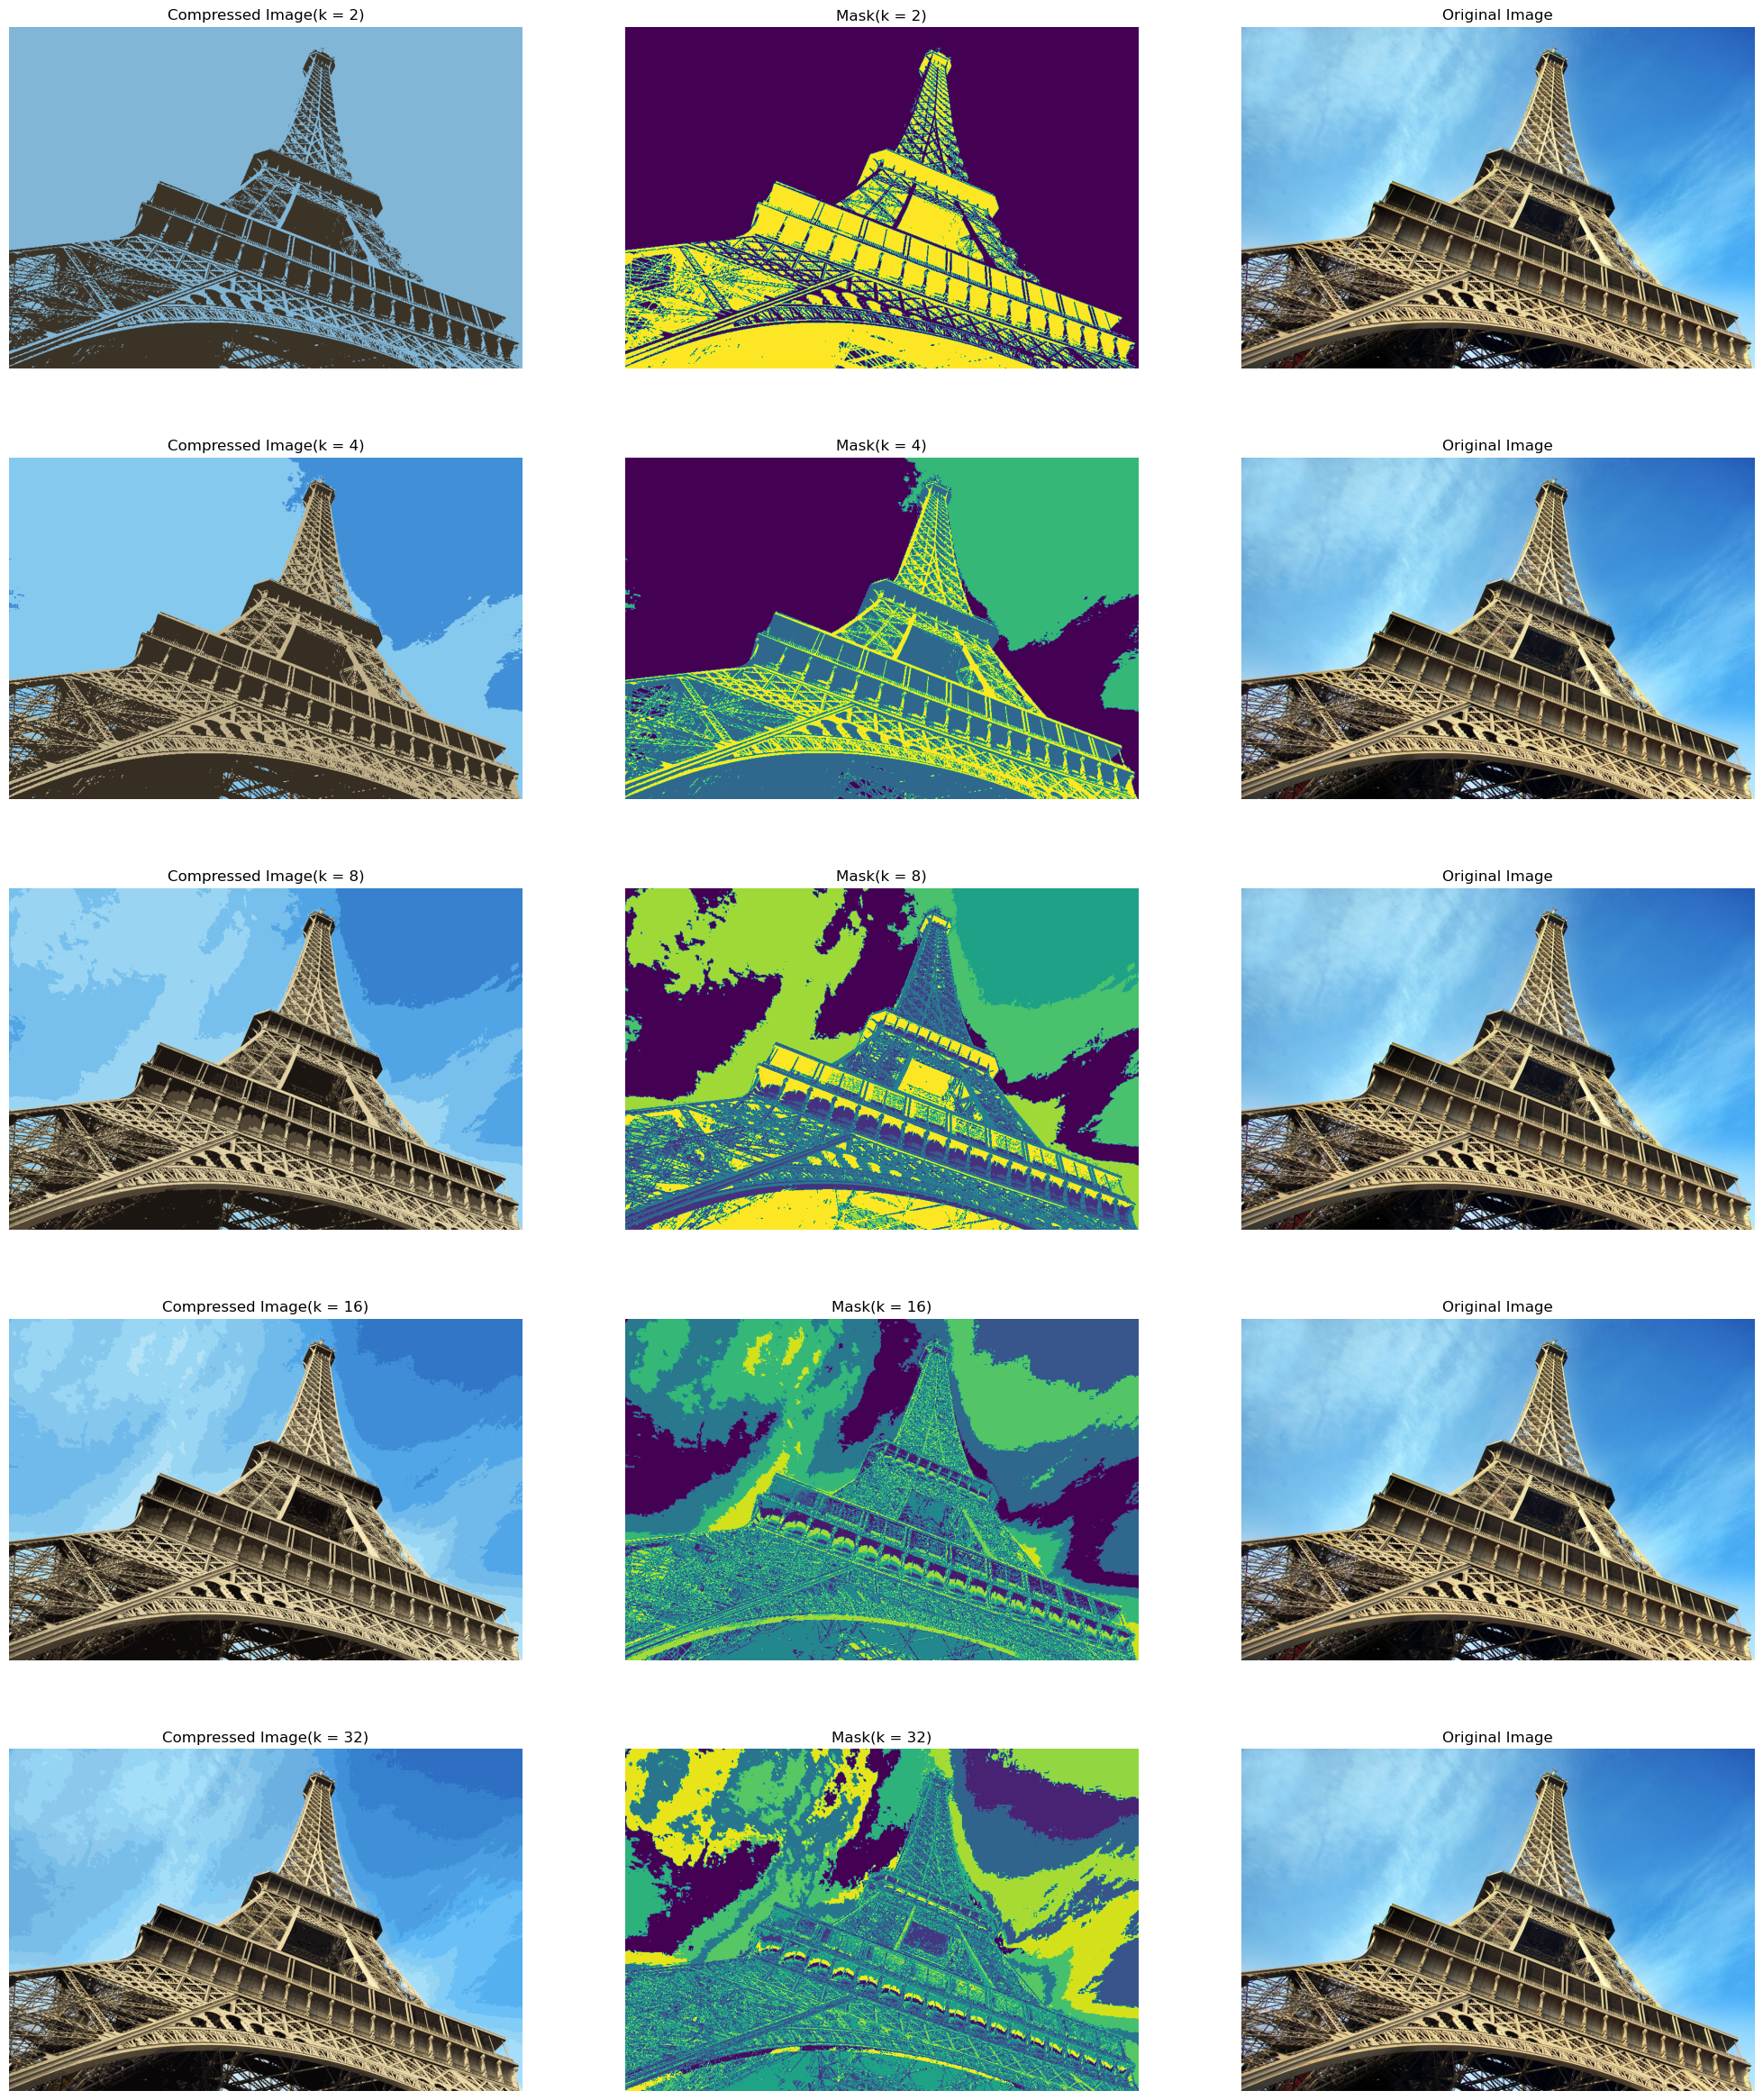
\includegraphics[scale=0.3]{figs/output.png}
	\caption{تصاویر همراه با ماسک تولیدی آنها، برای مقادیر مختلف $k$}
	\label{fig: dif k}
\end{figure}
\section{مقایسه سایز فایل تصاویر با مقادیر 
	$k$
	متفاوت
}
	سایز‌های مختلف برای مقادیر 
	$$k = 2, 4, 8, 16, 32$$
	در شکل 
	\ref{fig: dif size}
	نشان داده شده است
	\begin{figure}[H]
		\centering
		\includegraphics[scale=0.6]{figs/output1.png}
		\caption{سایز فایل تصاویر، برای مقادیر مختلف $k$}
		\label{fig: dif size}
	\end{figure}
	
	
	
	
	
	
	
	
	
	
	
	
	
	
	
	
	
	
	
	
\end{document}